\documentclass[10pt,a4paper]{article}
\usepackage[margin=1.6cm]{geometry}
\usepackage[latin1]{inputenc}
\usepackage{amsmath}
\usepackage{amsfonts}
\usepackage{amssymb}
\usepackage{multirow}
\usepackage{graphicx}
\usepackage{subcaption}

\setlength{\parskip}{5pt}
\setlength{\parindent}{0pt}

\author{Hector Dearman \and Paul Rowe-White \and Kritaphat Songsriin \and Simon Stuckemann}
\title{Machine Learning CBC: Neural Networks}
\begin{document}
\maketitle

\section{Implementation Details}
\subsection{Cross-Validation}
summary of implementation details, e.g. how we performed cross-validation

\subsection{Classification}
how we classified each example based on the 6 outputs, anything we think is important
flow chart

\subsection{Pre-processing and Post-processing}

\section{Evaluation Process}

\subsection{Finding Optimal Parameters (1)}
We assumed the parameters to be independent.
This is not a good assumption since the parameters are not necessarily independent however it is necessary to make the problem of optimising the parameters tractable.
We first set out each parameter we would have to optimise ???

To optimise a parameter we took the first fold of the data then for each value of the parameter we where trying we preformed three fold cross validation on that fold recording the average sum of the performance measure over each example in the validation set.
After doing this for each parameter value we selected the value with best performance measure

For most of the parameters it was possible to do a exhaustive (grid) search (after fixing a reasonable range and step size) however for the topology of the network, the number of layers and the number of nodes within each layer, it still proved impractical to try every combination.
We did two things to make optimising the topology possible in the time we had, we considered only topologies where every layer had the same number of nodes and we used a two layer search, first finding the best number of nodes to the nearest ten then we have a second search of the ten values on either side of the best result of the larger step\footnote{This will only be the true optimum value if the performance measure given the number of nodes is convex however so long as the larger step is smaller than large fluctuations in the performance measure this should do reasonably well.}.

???
- How we obtained the optimal parameters, topology
How should we be optimising parameters (not in the first fold only)
different topologies and parameters we experimented with

\subsection{Performance measure (1)}
Initially we used the classification error as a performance measure. 
This worked when we were building the six-output network however when we were building the one-output network this was difficult since you would like to train and optimise each individual network without having to guess whether the particular output it gave would be enough to classify an example.
We could have considered outputs less than 0.5 to be a negative classification however we would really like penalise or reward an output based on how right or how wrong it was.
Concretely if an example is labelled 0 and we predict 0.6 it's less bad (and our performance measure should give a better score) then if we predict 1.0. 

To do this we used the following logistic cost function:

\[
    Cost(p, y)= 
\begin{cases}
    -\log{p}& \text{if } y = 1\\
    -\log{(1 - p)}              & \text{if } y = 0
\end{cases}
\]

Where $p$ is the prediction for an example and $y$ is it's true label.
We take the sum of this cost function over every example in the validation set as our performance measure 
This new function gave very similar results to the previous measure on the six-output networks so we were confident it was not completely wrong.

\begin{figure}[!ht]
     \centering
     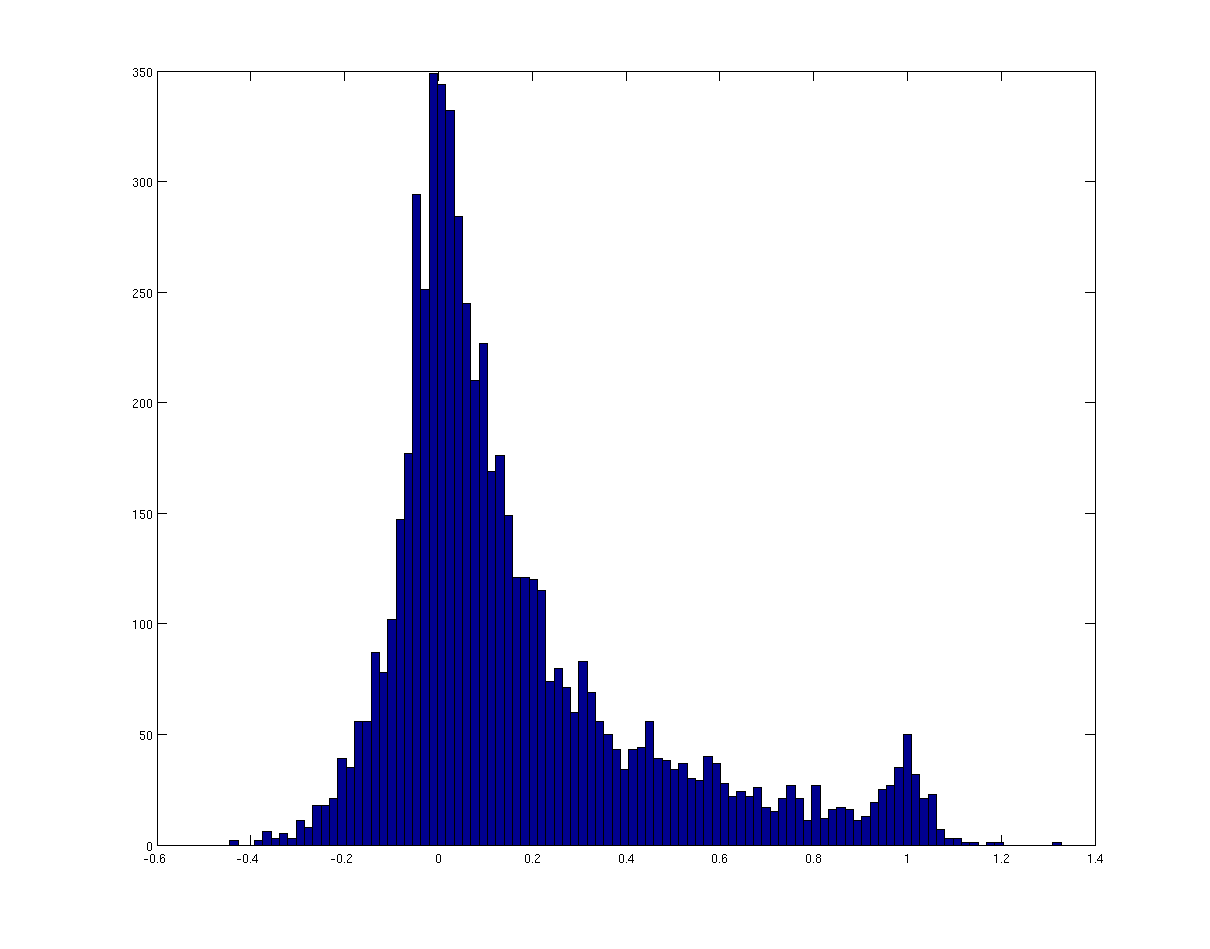
\includegraphics[width=\textwidth]{../../images/clean_hist.png}
     \caption{Histogram of Neural Network output}
     \label{fig:tree2}
\end{figure}


\subsection{Avoiding Overfitting (2)}
We used early stopping to avoid overfitting.
Early stopping is where we stop training if the error on the validation set starts increasing.
Specifically Matlab Neural Network Toolbox has a parameter {\tt max\_fail} which lets you specify a number of 
times the validation error can increase. 
After the validation error has increased {\tt max\_fail} times Matlab stops training and returns the weights which produced the lowest validation error so far.

An alternative approach is regularization, regularization modifies the performance function to encourage the network to produce smoother output.
This approach would again introduce a new parameter to optimise.
2

\section{Results (3)}

\begin{figure}[!ht]
     \centering
     \begin{subfigure}[b]{0.495\textwidth}
     	\includegraphics[width=\textwidth]{../../images/partially_optimised_everything.png}
     	\caption{???}
     	\label{fig:tree2}
     \end{subfigure}
     \begin{subfigure}[b]{0.495\textwidth}
     	\includegraphics[width=\textwidth]{../../images/partially_optimised_six_output_single_defaults.png}
     	\caption{???}
     	\label{fig:tree2}
     \end{subfigure}
\end{figure}


any difference between the average classification performance of the two types, both clean and noisy data. Discuss advantages and disadvantages

Commented results on average confusion matrices for both types of network and both clean and noisy with 
	- avg. classification rate
	- recall rate, precision rate, and F1 per class

figures of the average performance per fold for both types and nosiy/clean; discussion


\end{document}
 